\begin{block}{Distribution Estimation}
\centering
        \heading{Goal: Obtain the Best Distribution of $\lambda$} 
            {\large \textbf{Bayesian Context:} Simple Bayes model is insufficient, hierarchical Bayes model required.}
           
           {\large \textbf{Data Consistent Context:} Use data to construct observed distribution.}

        %\heading{Background}
             %{\large \emph{Data Consistent Inversion} is a Measure-Theoretic Framework for the solution of stochastic inverse problems. }
             
\end{block}


\begin{block}{Example}
\centering
$\begin{aligned}\prior\sim U[0,1]\end{aligned}$

Consider an exponential decay problem with uncertain decay rate:
\begin{equation*}
       u(t) = u_0\exp(-\lambda t), \; u_0 = 0.5 ,\; t=2
   \end{equation*}

\begin{tabular}{cc}
\multirow{3}{*}{\textbf{Simple Bayes}} & 
$\prior\sim U[0,1]$ \\
& $\likelihood\qGivelam \sim N\left(Q(\lam),\sigma^2\right)$ \\
                                        & $\bayes$ \\[2ex]
\textbf{Hierarchical Bayes} & $\Hbayes$\\
\textbf{Data Consistent \vspace{1cm} Inversion} & $\dci$ \\
\end{tabular}

\begin{figure}
        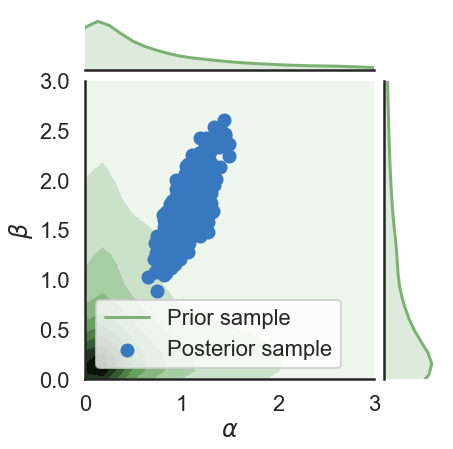
\includegraphics[width=5cm]{figures/distr_EX_hyper_param.png}
        \vspace{-0.5cm}
        \caption{ }
\end{figure}

\begin{figure}
        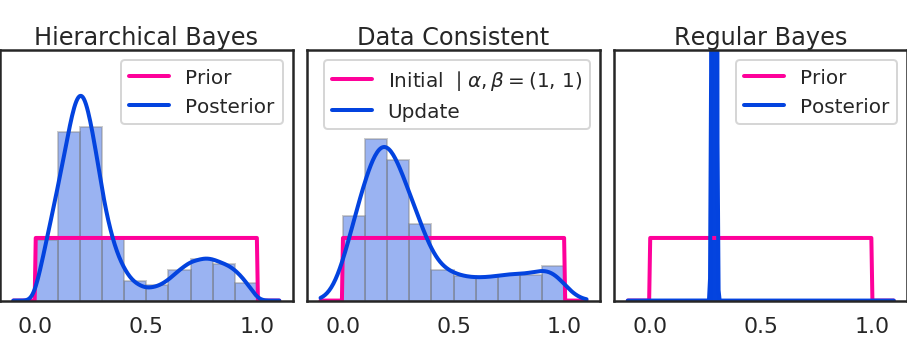
\includegraphics[width=30cm]{figures/distr_EX_lambda_space.png}
        \vspace{-0.5cm}
        \caption{ $\pspace$ Parameter Space }
\end{figure}
\begin{figure}
        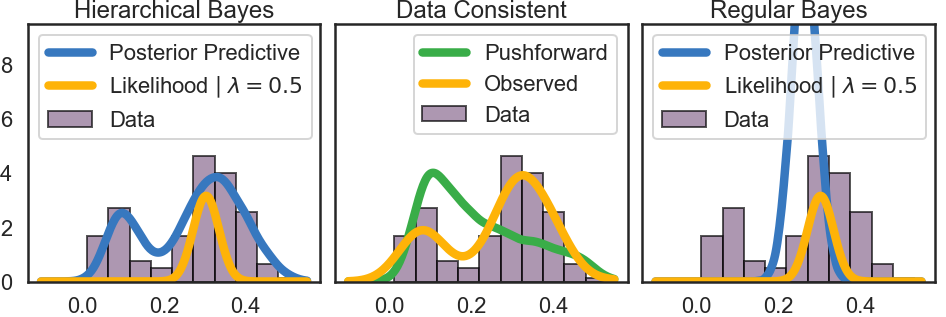
\includegraphics[width=30cm]{figures/distr_EX_data_space.png}
        \vspace{-0.5cm}
        \centering
        \caption{$\dspace$ Parameter Space  }
\end{figure}


\end{block}





\begin{block}{Takeaways}

\centering
\vspace{1cm}
    \heading{Data Consistent Inversion Performs Comparably with Hierarchical Bayes}
%     \begin{equation*}
%             \dciP \quad \vline \quad \dci
%     \end{equation*}
    %\begin{equation*}
    %        \dci
    %\end{equation*}
\begin{figure}
        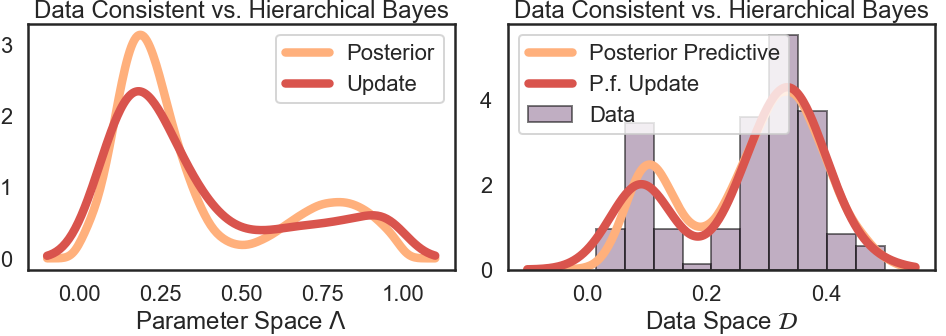
\includegraphics[width=30cm]{figures/distr_EX_comparison.png}
        \vspace{-0.5cm}
        \caption{ }
    \end{figure}
\end{block}
\heading{Non-parametric method with less sampling}
\heading{Future Research: How is it connected to Dirchlet Processes?}
